\section{Blockchain}
\subsection{Definizione di blockchain}
un ledger distribuito(libro mastro/contabilità) è un DB replicato su diversi nodi computazionali.
Ogni nodo ha una copa del ledger, ogni nodo che partecipa, si aggiorna autonomamente.
Non c'è un'autorità centrale, la blockchain è una forma delle tecnologie distribuite.

Una blockchain è:
\begin{itemize}
    \item un sistema che agisce come "fidato e terza parte", non centralizzato, sempre online, per mantenere un stato condiviso tramite scambi e computazioni sicure
    \item Un ledger distribuito, che salva i dati delle transazioni, raggruppate in blocchi e linkare i blocchi
    \item gestita da un grande gruppo di network servers
    \item full node: conserva una copia della blockchain, può create blocchi
    \item consensus: fra i full node, hanno gli stessi blocchi
    \item wallet: software per fare transazioni
    \item public = permissionless: tutti possono
        \begin{itemize}
            \item essere un utente
            \item fare transazioni
            \item partecipare al consenso
        \end{itemize}
    \item private = permissioned: le operazioni della blockchain possono essere fatte da membri autorizzati, full node identificabili, regole per l'accesso dei dati
\end{itemize}

\subsection{P2P Network}

I full node collaborativamente mantengono una rete p2p per lo scambio di blocchi e scambi di transazioni.

Le regole del consenso non coprono la parte di networking, i full node
possono usare protocolli orienteti alla velocità fra di loro le varie transazioni.

Al primo avvio di una applicazione, questa non consoce l'IP di nessun full node, effettua una query
ad un server DNS, questa query prende il nome di DNS seeds, che risponde all'applicazione con il lookup e
un indirizzo IP di un full node che accetta nuove connessioni.

Per validare una transazione, un full node deve aver scaricato tutti blocchi della blockchain per poter
aggiungere un nuovo blocco di transazioni.

Quando viene scoperto un nuovo blocco, questo viene inviato a tutti i peer della rete 
mediante la "Block Broadcasting".

\subsection{Motivi per usare una blockchain}
\begin{figure}[h!]
    \centering
    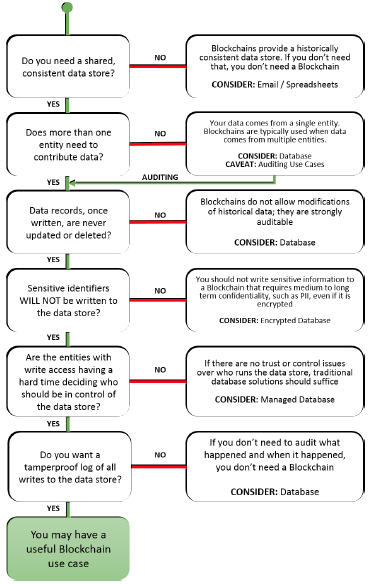
\includegraphics[width=0.5\linewidth]{imgs/14 - motivi uso blockchain.png}
    \label{fig:why_use_blockchain}
    \caption{Usi di una blockchain}
\end{figure}

\subsection{Coin vs Token}
Parlando di criptovalute associate a blockchain, si distinguono:
\begin{itemize}
    \item Coin: unità di valuta della blockchain, usata per le transazioni
    \item Token: unità secondaria che risiede nella blockchain con vari scopi:
        \begin{itemize}
            \item utility tokens: rappresentano il diritto di prendere prodotti/servizi dall'emittente del token
            \item security tokens: asset digitali il cui valore deriva da quanto questo asset viene scambiato
        \end{itemize}
\end{itemize}

Il security token potrebbe essere visto come "un'azione in borsa", può generare interesse, ecc


\subsection{Transazioni}
Le transazioni rappresentano pagamenti per beni o servizi utilizzando i "coins", 
le parti vengono identificate da chiavi pubbliche e 
ogni pagamento viee firmato digitalmente.

\subsection{Bitcoin}
\begin{itemize}
    \item Blocco di genesi: 3 Gennaio 2009
    \item developer: "Satoshi Nakamoto", Gavin Andresen, Wladimir van der Laan
    \item 1 BTC = $10^8$ satoshi
\end{itemize}

Le valte basate sulla blockchain, vengono generate tramite un processo decentralizzato e competitivo
detto mining.
I miners di bitcoin sono i full node che processano le transazioni e rendono sicuro il network.

C'è un numero limitato di bitcoin in circolo e i bitcoin vengono generati con un andamento 
prevedibile(mantenendo il prezzo stabile).

Visto che il marketcap di bitcoin è ancora piccole, quantità di denaro elevate possono far oscillare il prezzo.



\begin{figure}[h!]
    \centering
    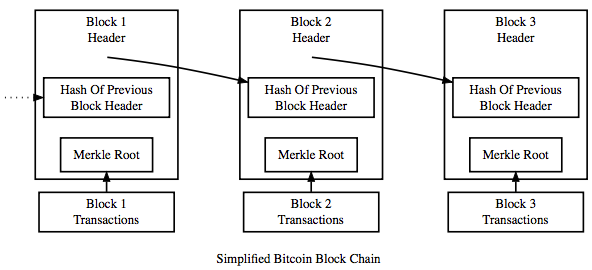
\includegraphics[width=0.5\linewidth]{imgs/15 - bitcoin block.png}
    \label{fig:bitcoin_block}
    \caption{Struttura Blocco bitcoin}
\end{figure}

Ogni blocco di transazioni, vengono "hashate" nel \textbf{Merkle tree}, finchè la hash unica(\textbf{Merkle Root}) 
viene prodotta e salvata nell'header del blocco, insiseme all'hash del header del blocco precedente.

\subsubsection{Merkle Tree}

\begin{figure}[h!]
    \centering
    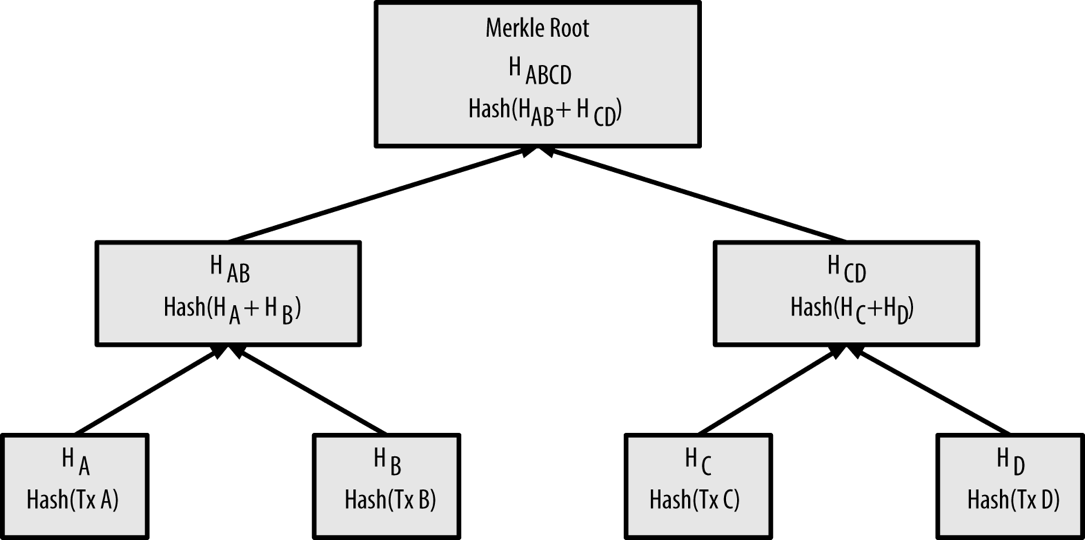
\includegraphics[width=0.5\linewidth]{imgs/16 - merkle tree.png}
    \label{fig:merkle_tree}
    \caption{Merkle Tree}
\end{figure}


Il merkle tree viene creato facendo l'hash di blocchi accoppiati (le foglie dell'albero),
Viene ripetuto il procedimento di pairing e hashing finchè non rimane una sola hash.

\subsubsection{Transazioni Bitcoin}
\begin{itemize}
    \item Tutte le transazioni sono collegate
    \item \textbf{input}: riferimeto al blocco precedente
    \item \textbf{output}: quantità di valuta da trasferire
    \item ogni transazioni ha più di un input e più di un output
    \item Se l'output è maggiore del'input, la transazione è annullata
    \item se il sender invia 50 ma il reciver vuole 25, ci saranno due transazioni da 25 di cui una sarà il "resto"
    \item il ricevitore invia la chiave pubblica al pagatore
    \item il pagatore crea la transazione, specificando l'output e la firma(hash della chiave pubblica del reciver)
    \item il payer firma la transazione con la propria chiave privata
    \item la transazione viene inviata dal sender alla rete di full node
    \item il full node verifica la transazione e se valida la aggiunge alla blockchain
\end{itemize}

\subsection{Smart contract}
\begin{itemize}
    \item Programma salvato nella blockchain
    \item espressione di logica contrattuale
    \item può implementare ogni algoritmo
    \item comportamento deterministico
    \item può interagire con altri contratti
    \item rende pubblica un'interfaccia
    \item può ritornare dati o salvare dati
    \item il messasggio può rappresentare eventi di interesse del contratto
    \item le interazioni con gli smartcontract sono salvate in blockchain
    \item DApp (applicazione decentralizzata): frontend + decentralized logic
    \item ICO (initial coin offering): crowfounding per un progetto, in cambio di coins specifici
    \item DAO (decentralized anonymous organization): organizzazione anonima amministrata da uno smart contract
\end{itemize}

\subsubsection{Concorrenza e smart contract}

\textbf{contracts-as-comcurrent-objects analogy}: account che usano gli smart contract in una blockchain sono come i threads di un pc.

\subsection{Ethereum}
\begin{itemize}
    \item Si può usare un'implemetazione di go
    \item 60 milioni di ether creti grazie ai contributori del presale
    \item 12 miglioni dati alla fondazione, ai finanizatori e ai dev
    \item 5 theters crati ogni blocco(13 sec per minare un blocco)
\end{itemize}

\subsubsection{Ethereum accounts}
Due tipologie di account in ethereum:
\begin{itemize}
    \item normale: controllato da coppie di chiave pubblica
    \item contratto: controllato dal codice interno
\end{itemize}

Chiavi private da 256 bit e pubbliche da 512 bit, vengono generate per ogni account.

\subsubsection{Smart contract ethereum}
Ogni smart contract ha un indirizzo unico, assegnato da una transazione speciale, dopo la quale, il programma fa parte della blockchain.
Per compie una interazione, bisogna mandare un messaggio all'indirizzo del contratto.
I contratti possono avere stato e memoria interna.

I contratti ethereum vengono scritti in \textbf{Solidity}(simile a javascript), compilato ed esequito nella ethereum virtual machine(EVM).

\begin{itemize}
    \item \textbf{kovan, ropsten}: testnet
    \item \textbf{truffle}: framefork(test i contratti in locale)
    \item \textbf{ganache}: crea una blockchain locale per test
\end{itemize}

Ogni operazione effettuta da un contratto, ha un costo.
\begin{itemize}
    \item TX = tassa totale operazione
    \item GU = gas usato per l'operazione
    \item GP = prezzo del gas
\end{itemize}

\begin{math}
    TX = GU * GP
\end{math}

E operazioni diverse hanno un consumo diverso di gas.

Il gas limit è il limite è il limite per il quale si è decisi di pagare.
Impostare un gas limit troppo alto risulta meno interessante per i miners, che cercano di massimizzare i guadagni per ogni songolo blocco.

I miner guardano il prodotto tra gas price e gas limit per vedere quale contratto è più remunerativo.

\subsubsection{Verifica di Merkle in ethereum}
In ETH, lo stato è un'enorme struttura dati chiamata \textbf{modified merkle patricia trie}, gli header di ogni blocco 
contengono tre merkle tree(transazioni, receipts(ricevute? e lo stato)).

\begin{figure}[h!]
    \centering
    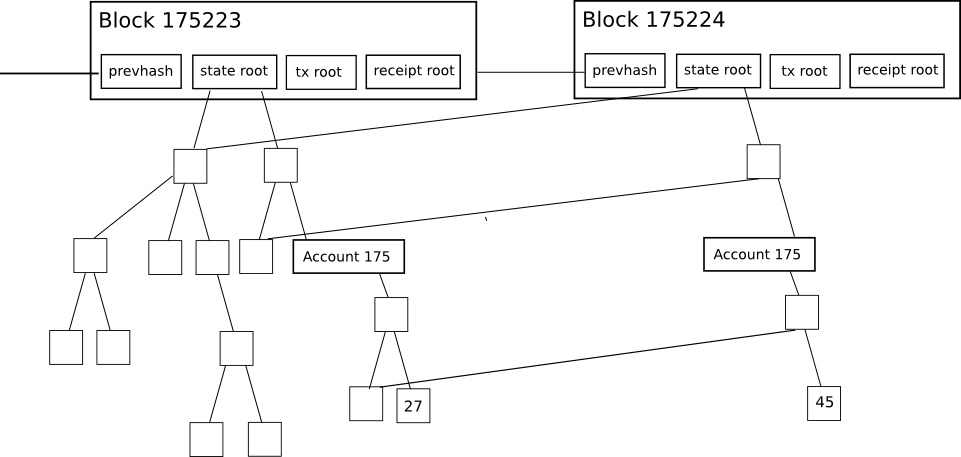
\includegraphics[width=0.5\linewidth]{imgs/17 - merkle tree.png}
    \label{fig:merkle_proof}
    \caption{Applciazione del Merkle tree}
\end{figure}

Bitcoin usa un albero binario, in ETH, usando l'albero di merkle si possono ottenere struttre molto complesse come
Transazioni richieste, transazioni in uscita e gli stati dell'account.

Si utilizaz il Merkle patricia tree perchè permette:
\begin{itemize}
    \item Calcolo facile del nuovo albero dopo la modifica
    \item La profondità dell'albero e vincolata
    \item la radice dipende solo dai dati(non l'ordine degli aggiornamenti)
\end{itemize}



\subsection{Modelli di consenso}
Principio importante della blockchain è chi è l'utente a creare un nuovo blocco.

In blockchain "permissionless", ci sono vari nodi che creano blocchi che competono per il blocco.
Fanno il nuovo blocco per vincere criptovalute.

Motivati dal guadagno.


Le seguenti proprietà sono in gioco:
\begin{itemize}
    \item Si parte dal blocco di genesi
    \item gli utenti sono daccordo con il modello di consenso sui blocchi creati
    \item ogni blocco è linkato al precedente mediante un hash
    \item ogni utente può verificare i blocchi.
\end{itemize}

I modelli di consenso comuni sono:
\begin{itemize}
    \item Proof of work
    \item Proof of Stake
    \item Round Robin
    \item Proof of Authority/Proof of Identity
    \item Proof of Elapsed Time
\end{itemize}

\subsubsection{Proof of Work(PoW)}
I full node competono a creare il nuovo blocco.
Spesso si utilizzano gli ASIC, PC specilizzati in fare coalcoli per la creazione dei blocchi.
Clacolano l'hash di alcuni dati finchè il risultato è simile alla traccia, il primo nodo che finisce l'operazione, propone il nuovo blocco nella blockchain.

Per ogni blocco aggiunto il full node prende una ricompensa in criptovalute.

La difficolta del problema di hash viene ricalcolato continuamente per mantenere lo stesso tempo stabile fra ogni blocco creato.


In Bitcoin, SHA-256 crea una hash del merkle tree + blocco precedente + header + random finchè il risultato non rispetta la soglia.

I nuovi blocchi vengono aggiunti solo se risolvere la loro hash era difficile quanto stabilito dal metodi di consenso.
Ogni N blocchi (N = 2016 in bitcoin), la sogni di difficoltà si ribilancia calcolando il tempo tra il primo e l'ultimo blocco.

In ETH l'algoritmo si chiama \textbf{Ethash}, la funzione per minare combina e fà l'hash (Keccak-256) di: random, hash dell'header del blocco e dati random del set.

L'algoritmo itera finchè la soglia non è raggiunta.

Il "Miner" che raggiunge l'hash di difficoltà accettata dalla soglia, prende la commissione, aggiunge il blocco alla blockchain e diffonde la notizia.

Non conviene aggiungere tante trasazioni in un blocco perchè rallenta la creazione del blocco.


Se qualcuno possiede il $51\%$ di hash rate della blockchain, potrebbe modificare le transazioni e evitare che nuove transazioni vengano fatte.

Se due nodi creano un blocco nello stesso momento, la chain si biforca e se nella blockchain 2 viene aggiunto un nuovo blocco, questa seconda chain diventa più affidabile della prima poichè più difficile da ricreare(ha un blocco in più).

\begin{figure}[!ht]
    \centering
    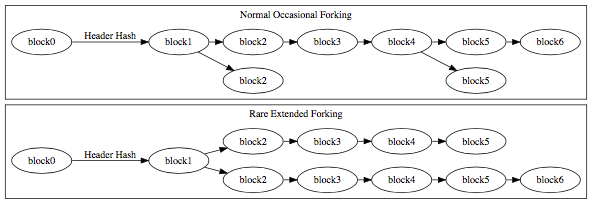
\includegraphics[width=0.5\linewidth]{imgs/18 - fork.png}
    \label{fig:fork}
    \caption{Biforcazione della blockchain}
\end{figure}

PoW è molto dispendiosa in quantità di energia.


\subsubsection{Proof of Stake(PoS)}

La blockchain mantiene proprietà di una popolazione di coins "staked" dai partecipanti.
Per aggiungere un blocco, la probabilità di creare un nuovo blocco aumenta se si hanno più coins in stacking.

Vantaggi:
\begin{itemize}
    \item minor rischio di centralizzazione
    \item efficienza energetica
\end{itemize}

Svantaggi:
\begin{itemize}
    \item eleggere il creatore del blocco implica randomicità
    \item brecce di sicurezza.
\end{itemize}

Gli attaccanti possono fare l'hash dell'intera blockchain per sferrare l'attacco "grinding attack".

\subsubsection{Eventual-consensus PoS protocols}
Questo protocollo applcia una forma di "longest-chain
rule" alla blockchain, l'immutabilità della blockchain aumenta con la quantità di blocchi.

\subsubsection{Blockwise-BA PoS protocols}
Questo protocollo ottiene l'immutabilità di ogni singolo blocco mediante il protocollo \textit{Byzantine Agreement}.

Esempio: ALGORAND


\subsubsection{Problema di non avere stacking}
Visto che la validazione dipende dallo stacking, non avere stacking porta problemi come la Biforcazione.

Portando a fenomeni come il double spending, competizione per blocchi su catene diverse ecc.

\subsubsection{Attacco a lungo termine}
Legato al concetto di creare "brench" senza sforzo, si riferisce alla capacità di alcuni set di stackholders di eseguire la blockchain
dal blocco di genesi e produrre una alternativa alla blockchain.

Due attacchi:
\begin{itemize}
    \item posterior corruption
    \item stake-bleeding
\end{itemize}

Per evitare i long range attack:
\begin{itemize}
    \item checkpoints: gli ultimi K blocchi possono essere riorganizzati
    \item valutazione della chiave crittografica
    \item restrixioni della densita della chain
\end{itemize}

\subsubsection{Blockchain $\approx$ Merkle hash function}
La struttura della blockchain è molto simile allo schema di merkle per la funzione di hash, dove la compressione è iterata su un messaggio che viene processato in blocchi.

La funzione di hash di Merkle deve soddisfare tre proprietà di sicurezza:
\begin{itemize}
    \item preimage resistance
    \item second preimage resistance
    \item collision resistance
\end{itemize}

\subsubsection{Eclipse attack}
L'attacco opera al livello della rete p2p, un nodo sotto attacco ottiene una vista distorta della blockchain perchè l'attaccante controlla le comunicazioni.

\subsubsection{Riassunto delle possibili falle di sicurezza}
PoW:
\begin{itemize}
    \item 51$\%$ attack
\end{itemize}

PoS:
\begin{itemize}
    \item Nothing at Stacke
    \item Long-Range attack
\end{itemize}

Problemi generali:
\begin{itemize}
    \item second preimage attack
    \item Eclipse attack
\end{itemize}

\subsubsection{Modello di consenso Round Robin}
Usato da network \textbf{Permissioned}, non ha puzzle crittografici e ha una potenza richiesta ridotta.
I nodi a turno creano i blocchi ed è presente un timeout per prevenire che nodi in "stallo" alterino la crescita della blockchain.

\subsubsection{Modello di consenso Proof of Authority/Proof of Identity}
I nodi che creano blocchi devono avere un'identità verificata e hanno una reputazione da preservare, minore è la reputazione, minore sono le possibilità di creare blocchi.
Utilizzabile solo nelle reti \textbf{permissioned}

\subsubsection{Proof of Elapsed Time(PoET)}
Ogni nodo richiede un timer di attesa all'\textbf{hardware time source}, l'hardware genera il tempo di attesa
e una volta ricevuto il timer, vanno in idle.
Una volta ripartito dall'idle, il nodo, crea un blocco, tutti gli altri blocchi interrompono l'idle e il processo riparte.

Utilizzabile in network \textbf{Permissioned e trusted}.